% A skeleton file for producing Computer Engineering reports
% https://github.com/DeepHorizons/KGCOEReport_template

\documentclass[CMPE]{KGCOEReport}

% !TEX outputFormat = pdf

\usepackage{indentFirst}
\usepackage{graphicx}
\usepackage{subcaption}
\usepackage{hyperref}
\usepackage{float}

\setlength{\parindent}{6mm}

\newcommand{\classCode}{CMPE 665}
\newcommand{\name}{Simon Kirkwood \& Adam Seidman}
\newcommand{\TAs}{Rohan Challa \& Prangon Das}
\newcommand{\LectureSectionNum}{1}
\newcommand{\LectureInstructor}{Muhammad Shaaban}
\newcommand{\exerciseNumber}{2}
\newcommand{\exerciseDescription}{Homework 2}
\newcommand{\submissionDate}{December 2, 2021}

\begin{document}
\maketitle

\setlength{\parskip}{1cm}

\section*{Abstract}

The goal of the assignment was to observe and analyze different partitioning methods 
for parallel programs via a ray tracing algorithm. Ray tracing is known for being highly 
parallelizable as each pixel of the image can be rendered entirely independently of 
the others, however the computation time of each pixel can vary wildly, so assigning 
pixels to separate processes in an efficient way is not a trivial task. Several different 
partitioning models were written and tested with the goal of comparing their performance 
and analyzing their strengths and weaknesses.

\section*{Design Methodology}

For each partitioning model to which orientation applies, the horizontal orientation 
will be described, with the knowledge that the same principles apply in reverse to the 
vertical orientation. The first model written will be referred to as "static strips". 
It involves using the number of processes on which the program is run to divide the 
image into that many equal-sized rows or columns, depending on orientation.

First, the vertical resolution of the image is divided by the number of processes in 
order to calculate the height of each row. Then, each process uses its rank number as 
an index to determine its starting row and ending row, which is its rank plus one. This 
is multiplied by the row height to get the actual pixel values. The last process rank 
has its stop row set to the last row of pixels instead, in the event that the resolution 
was not evenly divisible by the number of processes. The processes then iterate through 
each of the rows to which they are assigned, shading every pixel in those rows.

The second algorithm is referred to as "static blocks." It is similar in principle to 
static strips in that is involves dividing the image into equal-sized chunks, however 
in this case it is divided into a grid of squares. It should be noted that for this reason, 
the amount of processes must have a square root that is a positive integer, as the grid 
dimensions are calculated using this square root.

Once the grid dimensions have been calculated (the width being equal to the height), 
the value is used to calculate the width and height in pixels of each block. From that, 
the rows and columns for each process are calculated. The starting row of a process is 
its rank divided by the grid dimension, multiplied by the block height. The starting column 
is the remainder (modulo operation) of the rank divided by the block dimension, multiplied 
by the block width. The same iteration is then performed as with the static strips in 
order for each process to shade its assigned pixels.

The final static partitioning model is referred to as "static cycles." It revolves around 
splitting the image up into constant-sized rows/columns of which each process runs multiple. 
The process to which each strip is assigned follows a cyclical pattern so each process gets 
as close to an equal amount of strips as possible. It requires that the size of each cycle 
is defined as a command-line argument.

Using the predefined cycle size, each process uses its rank multiplied by the size as its 
starting row. Each time it loops, it adds this same value to itself in order to cycle to 
its next starting row. Within this loop, it goes row of pixels by row of pixels, shading 
each one across the entire width of the image. When the process has finished this for each 
cycle, it results in multiple thin separate strips of pixels going down the length of the image.

Every static model then has the same process for being combined. Each process send its shaded 
pixels to the master thread. The master thread then uses an identical algorithm to theirs, one 
by one, to determine for each process which pixels it was responsible for shading. It then 
takes each of those pixels and assigns its value to the master thread's own array of pixels. 
After doing this for every process in the communicator, the master thread has the complete 
image assembled, which it can then output to a file.

The dynamic partitioning model is designed to be slightly different. In this method, the user 
can supply command line arguments to determine the block sizes being sent to the worker 
processes. For this model, only the worker processes do pixel shading. The master process 
assigns blocks of pixels to the workers and when they are finished, it will assign them new ones. 
It keeps doing this until there are no blocks left to assign. Afterward, it waits until all 
other processes are finished and sends them a flag to tell them that they are done rendering 
the image. Each slave process then sends the pixels it rendered back to the master process, where 
they are reassembled into the main, final image.

\section*{Results/Analysis}

As a control group, sequential run times were measured for both the simple and complex scene. For 
the simple scene, a time of 168.24 seconds was recorded. The complex scene yielded a time 
of 5799.96 seconds. Each partitioning model's speedups are calculated in relation to these times.

The results of the first partitioning method, static strips, are shown in 
Table \ref{tab:static-strips-simple} and Table \ref{tab:static-strips-complex} for 
the simple and complex scenes respectively. \\

\begin{table}[!htpb]
\centering
\caption{\label{tab:static-strips-simple}Static vertical strips, rendering a simple scene.}
\begin{tabular}{ccccc}
\hline
\multicolumn{1}{l}{Processes} &
  \multicolumn{1}{l}{Number of Strips} &
  \multicolumn{1}{l}{Execution Time} &
  \multicolumn{1}{l}{Speedup} &
  \multicolumn{1}{l}{C-to-C ratio} \\ \hline
2 & 2 & 105.22 & 1.60 & 0.0040 \\
4 & 4 & 67.44  & 2.49 & 0.0122 \\
9 & 9 & 33.63  & 5.00 & 0.0490 \\
\end{tabular}
\end{table}

\vspace*{1mm}

The speedup for the simple scene is fairly strong with two processes, but the performance 
gain drops off as more processes are added. This is likely due to the scene having a 
variation in complexity for different parts of the scene, resulting in heavy load 
imbalance that puts much of the burden on relatively few processes. \\

\vspace*{1mm}

\begin{table}[!htpb]
\centering
\caption{\label{tab:static-strips-complex}Static vertical strips, rendering a complex scene.}
\begin{tabular}{ccccc}
\hline
\multicolumn{1}{l}{Processes} &
  \multicolumn{1}{l}{Number of Strips} &
  \multicolumn{1}{l}{Execution Time} &
  \multicolumn{1}{l}{Speedup} &
  \multicolumn{1}{l}{C-to-C ratio} \\ \hline
2 & 2 & 5393.56 & 1.08 & 0.00011 \\
4 & 4 & 3634.81 & 1.60 & 0.00014 \\
9 & 9 & 2964.91 & 1.96 & 0.00007 \\
\end{tabular}
\end{table}

\vspace*{1mm}

The same holds true for the complex scene, this time to a very great extent. Running 
the scene with two processes has a speedup of only 1.08, indicating that one of the 
processes had much more work to do than the other, and this applies to an even larger 
extent with more processes added. Based on these results, statically splitting the 
image into strips is not well suited to ray tracing.

The next method is static blocks, represented in Table \ref{tab:static-blocks-simple} 
and Table \ref{tab:static-blocks-complex}. For the complex scene, it should be noted 
that the cluster seemed to be stalling out during the time that it was attempted to 
be run with four processes, possibly due to a high volume of users at the time or 
some other issue, so only the results for nine processes were obtained.

\begin{table}[h]
\centering
\caption{Static blocks rendering a simple scene}
\label{tab:static-blocks-simple}
\begin{tabular}{ccccc}
\hline
Number of Processes & Number of Blocks & Execution Time & Speedup & C-to-C \\ \hline
4                   & 4                & 75.27          & 2.23    & 0.0249 \\
9                   & 9                & 52.19          & 3.22    & 0.0214
\end{tabular}
\end{table}

\vspace*{1mm}

The speedup for the simple scene was quite weak for this partitioning method as well, 
again likely due to a heavy load imbalance in the complexity of the scene. \\

\vspace*{1mm}

\begin{table}[h]
\centering
\caption{Static blocks rendering a complex scene}
\label{tab:static-blocks-complex}
\begin{tabular}{ccccc}
\hline
Number of Processes & Number of Blocks & Execution Time              & \multicolumn{1}{c}{Speedup} & \multicolumn{1}{c}{C-to-C} \\ \hline
9                   & 9                & \multicolumn{1}{r}{3095.73} & 1.87                        & 0.00034                   
\end{tabular}
\end{table}

The same once again holds true for the complex scene, to an even greater degree. The 
stark contrast in complexity between the edges of the scene and the center 
exemplify why this would occur.

For the last of the static methods, Table \ref{tab:static-cycles-simple}, 
Table \ref{tab:static-cycles-complex}, Table \ref{tab:static-cycles-simple-2} and 
Table \ref{tab:static-cycles-complex-2} represent results from the static cycles model.

\begin{table}[!htpb]
\centering
\caption{Static horizontal cycles, rendering a simple scene.}
\label{tab:static-cycles-simple}
\begin{tabular}{ccccc}
\hline
\multicolumn{1}{l}{Processes} &
  \multicolumn{1}{l}{Height of Strip} &
  \multicolumn{1}{l}{Execution Time} &
  \multicolumn{1}{l}{Speedup} &
  \multicolumn{1}{l}{C-to-C ratio} \\ \hline
4 & 1    & 48.27 & 3.48 & 0.0181  \\
4 & 5    & 48.09 & 3.49 & 0.0173  \\
4 & 10   & 48.44 & 3.47 & 0.0178  \\
4 & 20   & 48.45 & 3.47 & 0.0191  \\
4 & 80   & 48.88 & 3.44 & 0.0181  \\
4 & 320  & 50.11 & 3.35 & 0.0174  \\ 
4 & 640  & 54.36 & 3.09 & 0.0158  \\
4 & 1280 & 82.78 & 2.03 & 0.0108  \\ \hline
9 & 1    & 22.89 & 7.34 & 0.0894  \\
9 & 5    & 22.79 & 7.38 & 0.0862  \\
9 & 10   & 22.72 & 7.4  & 0.085   \\
9 & 20   & 22.41 & 7.5  & 0.0805  \\
9 & 80   & 21.99 & 7.65 & 0.0859  \\
9 & 320  & 29.34 & 5.73 & 0.0565  \\
9 & 640  & 46.11 & 3.64 & 0.0194  \\
9 & 1280 & 81.27 & 2.07 & 0.0141 
\end{tabular}
\end{table}

The cyclical model marks a significant improvement in speedup, for a sufficiently 
small cycle size. Because of the nature of the cycles, it is better at distributing 
the complex parts of the image out more evenly, so each process has a more equal 
amount of work to accomplish. This causes less time to be wasted, and therefore 
the entire execution finishes more quickly. This effect is lessened with larger 
cycle sizes because the image is broken up into chunks which are more likely to 
be separate in terms of complexity.

It should also be noted that with a cycle size high enough, there are not enough cycles 
to even assign to all 9 processes, so some go entirely without a workload in those 
cases, dramatically influencing the speedup negatively. \\

\vspace*{1mm}

\begin{table}[!htpb]
\centering
\caption{Static horizontal cycles, rendering a complex scene.}
\label{tab:static-cycles-complex}
\begin{tabular}{ccccc}
\hline
\multicolumn{1}{l}{Processes} &
  \multicolumn{1}{l}{Height of Strip} &
  \multicolumn{1}{l}{Execution Time} &
  \multicolumn{1}{l}{Speedup} &
  \multicolumn{1}{l}{C-to-C ratio} \\ \hline
4 & 1    & 1490.41 & 3.89 & 0.00057 \\
4 & 5    & 1547    & 3.74 & 0.00053 \\
4 & 10   & 1520.3  & 3.81 & 0.00033 \\
4 & 20   & 1687.25 & 3.43 & 0.00018 \\
4 & 80   & 1773.2  & 3.27 & 0.0005  \\
4 & 320  & 3173.03 & 1.82 & 0.00027 \\ 
4 & 640  & 3012.96 & 1.92 & 0.00029 \\
4 & 1280 & 3599.4  & 1.61 & 0.00014 \\\hline
9 & 1    & 666.66  & 8.7  & 0.00251 \\
9 & 5    & 687.04  & 8.44 & 0.00173 \\
9 & 10   & 729.27  & 7.95 & 0.00085 \\
9 & 20   & 779.82  & 7.43 & 0.00229 \\
9 & 80   & 1130.73 & 5.12 & 0.00123 \\
9 & 320  & 2612.4  & 2.22 & 0.00063 \\
9 & 640  & 3014.53 & 1.92 & 0.0003  \\
9 & 1280 & 3613.55 & 1.6  & 0.00031
\end{tabular}
\end{table}

\vspace*{1mm}

The same analysis applies to the complex scene once again. Its more dramatic 
differences in complexity between different areas of the scene accentuate 
these effects even more. Figure \ref{fig:graph_cyclical} shows the comparison 
between cycle size and execution time for both four and nine processes. Once 
the cycle height reaches 640, it can be seen that more processes become 
virtually useless.

\begin{figure}[H]
  \centering
  \begin{subfigure}[b]{0.85\linewidth} % scale 0.9
    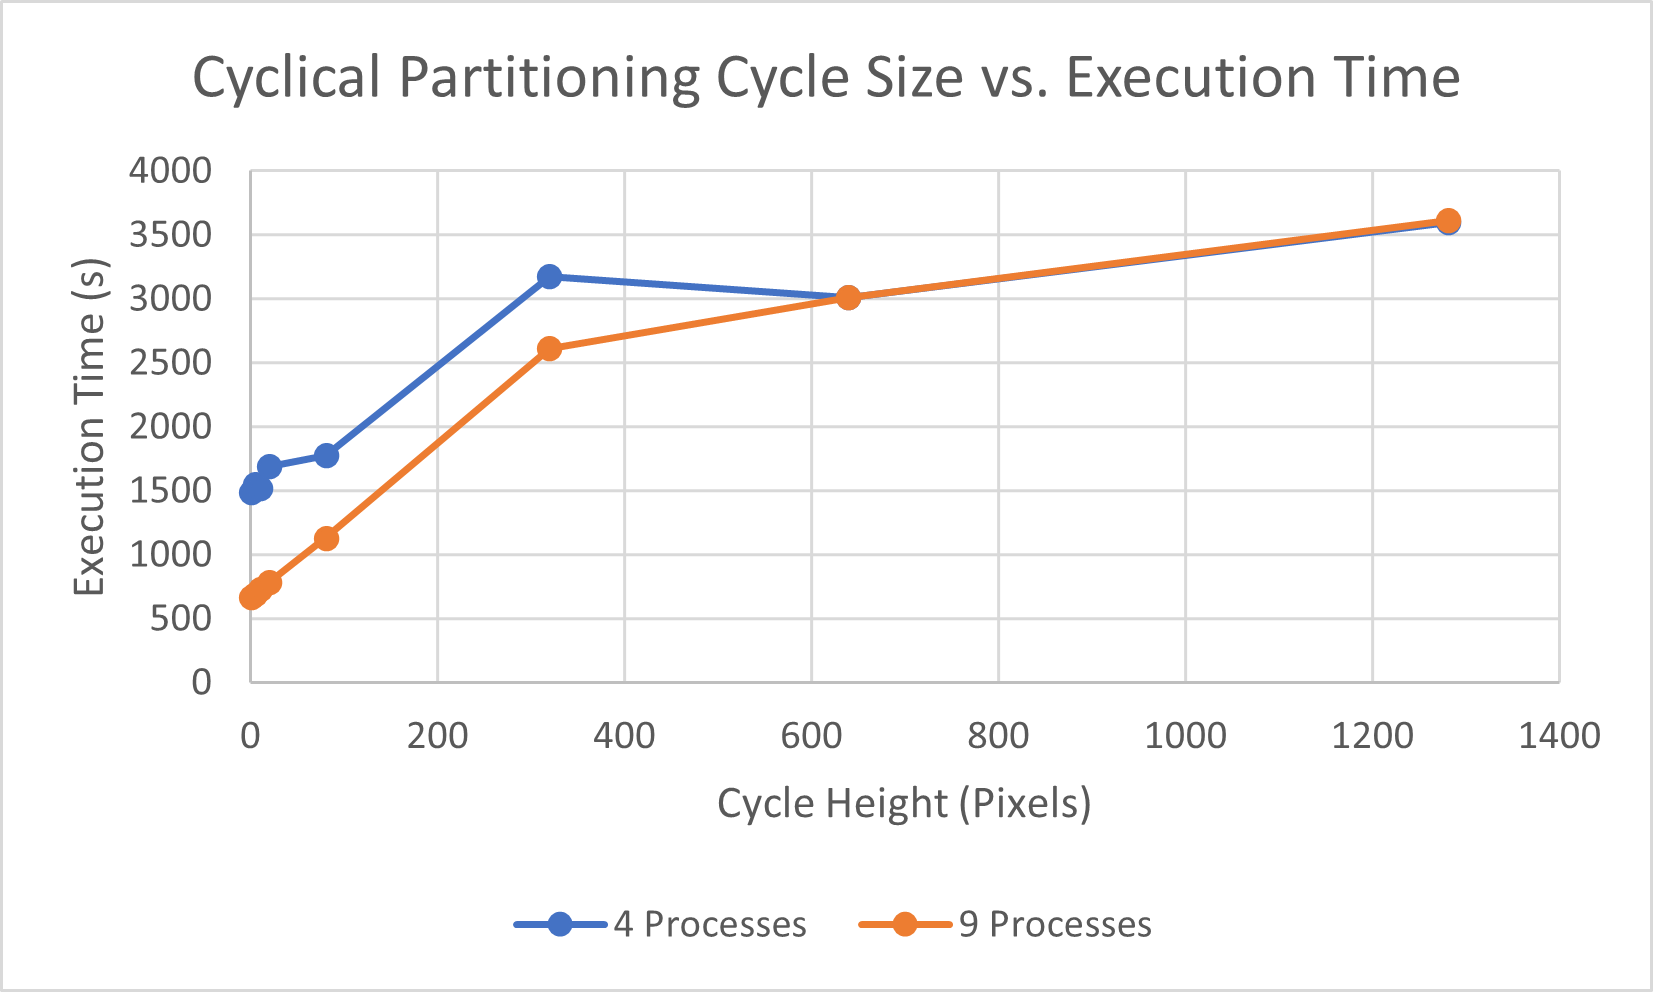
\includegraphics[width=\linewidth]{GraphCyclical.png}
  \end{subfigure}\\
  \caption{ \textit{Comparison of cycle sizes with 4 and 9 processes.}}
  \label{fig:graph_cyclical}
\end{figure}

The actual cause of this is somewhat vague. A cycle size of 640 should 
result in up to eight processes continuing to provide speedup, yet 
this strangely seems not to be the case. Of course, for a cycle size 
of 1280, the cause of a lack of speedup is quite evident. \\

\begin{table}[h]
\centering
\caption{Parallelism of static cycles with constant cycle size}
\label{tab:static-cycles-simple-2}
\begin{tabular}{ccccc}
\hline
\multicolumn{1}{l}{Processes} & \multicolumn{1}{l}{Cycle Size} & \multicolumn{1}{l}{Execution Time} & Speedup & C-to-C \\ \hline
2 & 27 & 94.38 & 1.78 & 0.0042 \\
4 & 27 & 48.01 & 3.50 & 0.0182 \\
9 & 27 & 22.65 & 7.43 & 0.0611
\end{tabular}
\end{table}

This table and Table \ref{tab:static-cycles-complex-2} below are meant to 
illustrate how well the partitioning model scales with additional processes. 
Higher amounts of processes could not be run due to an issue with the cluster, 
however the few examples that could be taken illustrate that it scales 
quite well with additional processes, with the number of processes and the 
speedup being fairly proportional. \\

\begin{table}[H]
\centering
\caption{Parallelism of static cycles with constant cycle size rendering a complex scene}
\label{tab:static-cycles-complex-2}
\begin{tabular}{ccccc}
\hline
\multicolumn{1}{l}{Processes} & \multicolumn{1}{l}{Cycle Size} & \multicolumn{1}{l}{Execution Time} & Speedup & C-to-C \\ \hline
2 & 27 & 2953.61 & 1.96 & 0.00019 \\
4 & 27 & 1594.17 & 3.64 & 0.00036 \\
9 & 27 & 808.642 & 7.17 & 0.00052
\end{tabular}
\end{table}

This once again holds true for the complex scene.

Dynamic partitioning worked quite well. As discussed earlier, the scenes can 
have dramatically different amounts of complexity depending on what is in 
each particular pixel. As a result, having a model that dynamically assigns 
groups of pixels can be very useful for keeping the load imbalance small. 
Table \ref{tab:dynamic-simple} and Table \ref{tab:dynamic-complex} show the 
results from this model.

Unfortunately, the 1x1 block size actually seemed to result in a segmentation 
fault, possibly due to too much memory being needed to store references to 
all the work units. This is a design flaw that could not be fixed in time and 
unfortunately caused results for that particular configuration to be unobtainable.

\vspace*{1mm}

\begin{table}[h]
\centering
\caption{Dynamic partitioning rendering a simple scene}
\label{tab:dynamic-simple}
\begin{tabular}{ccccc}
\hline
Processes & Block Size & Execution Time & Speedup & C-to-C \\ \hline
9 & 1x1     & N/A    & N/A  & N/A \\
9                   & 15x15      & 26.12          & 6.44    & 0.0118 \\
9                   & 25x25      & 26.42          & 6.37    & 0.0114 \\
9                   & 50x50      & 26.17          & 6.43    & 0.0120 \\
9                   & 75x75      & 26.14          & 6.44    & 0.0113 \\
9                   & 100x100    & 26.04          & 6.46    & 0.0117
\end{tabular}
\end{table}

\vspace*{1mm}

As expected, the dynamic model is great at reducing load imbalance as thus 
provides very impressive results. However, since it could only be run with 
nine processes, and not sixteen or thirty-six due to aforementioned cluster 
issues, the master thread not doing any calculations was actually a significant 
hamper on the speedup, proportionally speaking. As such, the speedup is 
actually slightly lower than for cycles. However, it could be expected that 
with a higher process count this effect would become less and less significant 
and dynamic partitioning would become the victor in terms of very high scaling.

\vspace*{1mm}

\begin{table}[h]
\centering
\caption{\label{tab:dynamic-complex}Dynamic partitioning rendering a complex scene.}
\begin{tabular}{ccccc}
\hline
Processes & Block Size & Execution Time & Speedup  & C-to-C                  \\
\hline
9 & 1x1     & N/A    & N/A  & N/A \\
9 & 15x15   & 739.35 & 7.84 & 0.00041 \\
9 & 25x25   & 760.22 & 7.63 & 0.00037 \\
9 & 50x50   & 800.29 & 7.25 & 0.00031 \\
9 & 75x75   & 791.92 & 7.32 & 0.00035 \\
9 & 100x100 & 848.04 & 6.84 & 0.00034
\end{tabular}
\end{table}

\vspace*{1mm}

As expected, a model that is the best at minimizing load imbalance would excel 
for a complex scene such as this one. The speedups are very strong, but dip 
slightly with larger block sizes which increase load imbalance somewhat.

Generally, the static cycles model seems to be best for lower process counts. 
With many more processors available, however, the dynamic partitioning would 
likely scale better and provide a better speedup as a result since its load 
balancing cannot be matched.

\section*{Conclusion}

The results of the exercise were successful, as they illustrated the 
clear differences in efficiency and scalability between different partitioning models. 
Through implementing and testing four different models, the requirements of scaling 
a raytracing algorithm become fairly evident. It also showcases a very prominent 
real-world example of parallelization which helps put the learned concepts into a 
better perspective. The issue with the cluster made the scope of the results 
limited, but this did not stop the data from showing some clear and illustrative patterns.

\end{document}
